\chapter{Lezione1}

\section{Introduzione}
La Fisica è la  scienza che studia i componenti della materia e le loro interazioni. Quello che ci interessa per poter affrontare il corso, sono le leggi fisiche.

Le leggi fisiche sono delle \textbf{relazioni quantitative tra grandezze.} In particolare, sono relazioni ricavate da esperimenti fatti  in laboratorio,  in  condizioni controllate, che riproducono i fenomeni naturali.

A livello pratico,  possiamo dire che le leggi fisiche sono relazioni matematiche (equazioni).

\subsection{Le misure}
Possiamo definire le misure come il \textbf{risultato di una procedura, in cui facciamo il confronto tra una grandezza e uno standard (o campione).}

\subsubsection{Le grandezze fondamentali}
In fisica sono state definite alcune grandezze fondamentali.  Per il corso ci interessano:
\begin{itemize}
	\item Lunghezza (misurata in metri)
	\item Tempo (misurato in secondi)
	\item Massa (misurata in chilogrammi)
	\item Intensità di corrente elettrica (misurata in ampere)
\end{itemize}

Abbiamo detto che le leggi fisiche sono delle equazioni; la prima cosa da verificare per la correttezza di tali equazioni è che,  a livello di unità di misura,  le grandezze che compaiono nel primo membro dell'equazione devono avere la stessa unità di misura di quelle che compaiono nel secondo membro. 

\subsection{Notazione per le misure}
I valori numerici che sostituiremo all'interno delle equazioni delle leggi fisiche, derivano da delle misure.  Tutte le misurazioni che facciamo,  hanno una precisione finita che dipende da quante cifre significative scriviamo quando riportiamo i risultati.

Per convenzione, l'ultima cifra significativa \textbf{corrisponde alla prima cifra affetta da incertezza.}

Supponiamo ad esempio, di avere una lunghezza  \textit{l} misurata in metri:
$$ l = 1.0\textbf{0} m $$ 
L'ultima cifra significativa è lo zero riportato in grassetto (il simbolo .  è la virgola). 
Il fatto che l'ultima cifra significativa è affetta da incertezza, significa che:
se chiamo $\Delta l$ l'incertezza con cui conosco questo valore, allora posso dire che 
$$\Delta l =  \pm 0.01m$$
Detto a parole, la precisione con cui conosco questo valore è più o meno $0.01m$

\subsubsection{Esempio 2}
$$ l^{1} = 5.0\textbf{0} m $$
 (la cifra affetta da incertezza è riportata in grassetto)
 
 Anche in questo caso, vediamo che l'incertezza è uguale a:
 $$ \Delta l^{1} = \pm 0.01m $$
 
 \subsection{La notazione scientifica}
 I valori numerici,  molto spesso, vengono riportati utilizzando la \textbf{notazione scientifica}. 
 
 Scrivere in questo modo, significa scrivere un numero in cui c'è una sola cifra diversa da zero prima della virgola, moltiplicata per un'opportuna potenza di 10.
 
 \subsubsection{Esempio con una lunghezza \textit{l}} 
 $$ l = 350\textbf{0}m$$
 Applicando quanto visto finora, possiamo affermare che:
 $$\Delta l = \pm 1m$$
 Se voglio esprimere la lunghezza \textit{l} in notazione scientifica devo scrivere:
 $$ l = 3.5 \times 10^{3}m$$
 Questa notazione però, non è del tutto corretta; scrivendo così,  infatti, vorrebbe dire che la prima cifra affetta da incertezza \textbf{non} sarebbe più lo 0 ma il 5
 
 In realtà il modo corretto di scrivere questo numero è
 $$ l = 3.500 \times  10^{3} m$$
 
\subsection{La precisione nei calcoli}
Quando lavoriamo con questi numeri, dato che sono dei reali, facciamo le classiche operazioni a cui siamo abituati come somma, prodotto ecc. La regola generale è che, quando si fanno operazioni di questo tipo, i\textbf{l risultato finale non può portare ad un aumento della precisione rispetto ai valori da cui siamo partiti.}

\subsubsection{Esempio con somme e sottrazioni}
Supponiamo di avere due lunghezze:
$$ l_{1} = 125\textbf{8}m  \quad l_{2} = 65.\textbf{4}m $$
Calcoliamo l'incertezza di queste due lunghezze:
$$ \Delta l_{1} = \pm 1m  \quad \Delta l_{2} = \pm 0.1m $$
Supponiamo, adesso, di voler determinare quanto valgono la lunghezza totale e l'incertezza totale:
$$ l_{tot} = l_{1} + l_{2} = 131\textbf{3}.4m $$
Per quanto riguarda l'incertezza totale, bisogna fare attenzione a non confondersi. Come detto prima, il risultato finale \textbf{non può portare ad un aumento della precisione.} Siccome la precisione con cui conosciamo i dati iniziali è determinata da quella con cui la conosciamo peggio (in questo caso $l_{1}$ perché ha un'incertezza maggiore), quando faremo la somma, il risultato sarà conosciuto anch'esso con una precisione
$$ \Delta l_{tot} = \pm 1m $$
Infatti,  per $l_{tot}$ la prima cifra significativa affetta da incertezza non è più il 4 dopo la virgola, ma è il 3 in grassetto; per questo motivo, volendo essere precisi, il valore corretto da scrivere è
$$ l_{tot} = 131\textbf{3}m \quad  \Delta l_{tot} = \pm 1m $$

\subsubsection{Esempio con prodotti e divisioni}
Anche con prodotti e divisioni, vale la regola generale vista sopra (non è così ovvio). Un caso tipico in cui si fa un prodotto, per esempio, è quando conosciamo il raggio di una circonferenza, e vogliamo calcolare la lunghezza della circonferenza stessa.

Come caso pratico, possiamo prendere il raggio della Terra, per poi calcolare la lunghezza della sua circonferenza (ipotizzando però, che la Terra sia una sfera perfetta).

Sia $ R_{Terra}$ il raggio della Terra; se lo conosco, allora la circonferenza della Terra è uguale a
$$ C_{Terra} = 2 \pi \cdot R_{Terra}$$
Se noi utilizziamo la calcolatrice, possiamo conoscere il valore di $\pi$ con diverse cifre decimali ($\pi = 3.14156$ ecc). Il punto è, però, che se conosciamo il raggio della Terra ad esempio a 10\textit{km}, chiaramente la circonferenza della Terra che determineremo con l'espressione vista sopra, non la conosciamo (per esempio) alla precisione del metro. Sappiamo che 
$$ R_{Terra} \approx 6.3\textbf{7 }\cdot 10^{6}m \quad  \Delta R_{Terra} = \pm 0.01 \times 10^{6} m = \pm 10km $$
Questo fa vedere, appunto, che la circonferenza della Terra la conosciamo al meglio di 10\textit{km} e non al meglio del metro.

La regola generale quando abbiamo prodotti e divisioni è che i\textbf{l numero di cifre significative presenti nel risultato, deve essere uguale al numero di cifre significative presenti nel termine che è conosciuto con la precisione peggiore.}

Riprendendo l'esempio sopra, il valore di $\pi$ lo conosciamo con quante cifre significative vogliamo, mentre il raggio della Terra lo conosciamo con tre cifre significative; ha senso,  quindi riportare la circonferenza della Terra con 3 cifre significative.


\section{Scalari e vettori}
In fisica ci sono due tipi di grandezze: gli \textbf{scalari} e i \textbf{vettori}.

Le grandezze scalari, sono grandezze fisiche che per essere specificate, richiedono di indicare un solo numero reale. Un esempio di grandezza scalare è la \textbf{temperatura}; quando diciamo che la temperatura in un certo punto è di\textbf{ 20°}, solamente utilizzando questa affermazione, abbiamo completamente specificato questa grandezza fisica. Visto che gli scalari sono numeri reali, per combinare tra di loro queste grandezze, abbiamo a disposizione le operazioni a cui siamo abituati fin dalle elementari (somme, prodotti...).

I vettori, invece, sono grandezze fisiche che, per essere specificate, oltre a richiedere un numero, che rappresenta l'intensità di tali grandezze, richiedono anche una \textbf{direzione} e un \textbf{verso}.

Un esempio tipico di grandezza vettoriale è lo \textbf{spostamento}. Supponiamo di essere in un punto del piano; se vogliamo dire di quanto ci spostiamo da questo punto, non basta semplicemente dire che ci siamo spostati (ad esempio) di \textit{10cm}. Per specificare correttamente questa grandezza, infatti, devo anche dire la direzione in cui mi sto spostando (per esempio orizzontalmente); infine devo specificare anche il verso (destra o sinistra). 

\begin{figure}[h]
\begin{center}
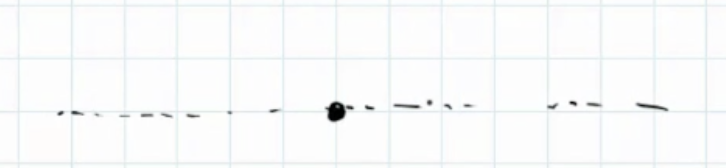
\includegraphics[width = 0.5 \textwidth]{lezione1/images/direzione.png}
\caption{Punto che si sposta in direzione orizzontale}
\label{fig:direzione}
\end{center}
\end{figure}

Ovviamente, devo specificare il verso, anche nel caso in cui mi sposto in direzione verticale.

Più precisamente, l'intensità di una grandezza vettoriale, (il numero reale), viene chiamata \textbf{modulo}.

Ricapitolando, quindi, per definire un vettore devo dare \textbf{modulo}, \textbf{direzione} e \textbf{verso}. 

Graficamente i vettori vengono rappresentati come un \textbf{segmento orientato di retta},  dove:
\begin{itemize}
\item utilizziamo un \textbf{segmento} perché il modulo è una quantità finita
\item \textbf{orientato} perché dobbiamo specificare un verso
\item la \textbf{retta} rappresenta invece la direzione
\end{itemize}

\begin{figure}[h]
\begin{center}
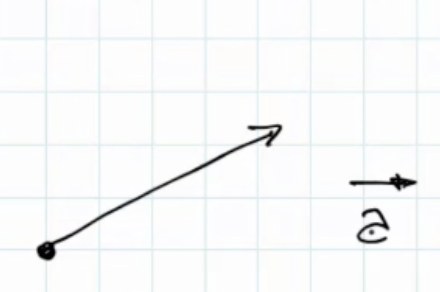
\includegraphics[width = 0.5 \textwidth]{lezione1/images/vettore 1.png}
\caption{Rappresentazione grafica di un vettore}
\label{fig:vettore 1}
\end{center}
\end{figure}
Il vettore sopra rappresentato si chiama $\overrightarrow{a}$
\subsection{Notazione}
Il modulo di un vettore viene indicato con $\left | \overrightarrow{a} \right |$ oppure
$\left | \left | \overrightarrow{a} \right | \right |$ per semplicità, visto che il modulo rappresenta la grandezza del vettore, noi lo indicheremo con $a$ senza la freccia sopra.

\subsection{Versore}
Il \textbf{versore è un vettore che ha modulo uguale a 1.} Visto che il vettore così definito ha modulo pari a 1, le uniche cose che ci interessano realmente di un versore sono la sua direzione e il suo verso.

\subsection{Prodotto di uno scalare per un vettore}
Sia $\overrightarrow{a}$ un vettore e $m$ uno scalare. Il prodotto di uno scalare per un vettore, restituisce un vettore (in questo esempio chiamato $\overrightarrow{b}$), fatto nella seguente maniera: $$ \overrightarrow{b} = m \cdot \overrightarrow{a} $$
Inoltre:
\begin{itemize}
	\item $b = \left | m \right | \cdot a $ cioè il modulo di $\overrightarrow{b}$ è uguale al modulo di $\overrightarrow{a}$ moltiplicato per il valore assoluto dello scalare $m$
	\item la direzione di $\overrightarrow{b} $ è la stessa di $\overrightarrow{a}$
	\item il verso di $\overrightarrow{b}$ è:
	\begin{itemize}
		\item lo stesso se $ m \geqslant 0 $
		\item l'opposto se $ m < 0 $
	\end{itemize}
\end{itemize}

\subsection{Trovare il versore di un vettore}
Abbiamo detto che un versore è un vettore di lunghezza unitaria che rappresenta una direzione e un verso.

Sia $ \overrightarrow{a} $ un vettore dato. Vogliamo, adesso, trovare il versore che rappresenta la direzione e il verso in cui è diretto $ \overrightarrow{a} $ 

Per farlo, dobbiamo scrivere un vettore che ha:

\begin{itemize}
	\item modulo uguale a 1
	\item direzione e verso uguali a quelli di $ \overrightarrow{a} $
\end{itemize}

Più semplicemente, se abbiamo un vettore $ \overrightarrow{a} $ possiamo sempre scriverlo come: il prodotto tra uno scalare uguale al modulo di $ \overrightarrow{a} $ moltiplicato per un versore $ \overrightarrow{u} $ che ha la stessa direzione e lo stesso verso di $\overrightarrow{a} $.
$$ \overrightarrow{a} = a \overrightarrow{u} $$

A questo punto, se vogliamo trovare il versore di $\overrightarrow{a}$ basta sfruttare l'equazione scritta sopra nel modo seguente:
$$ \overrightarrow{a} = a \overrightarrow{u} \Rightarrow \overrightarrow{u} = \frac{1}{a} \overrightarrow{a} $$

Detto a parole, per trovare il versore di $ \overrightarrow{a} $ dobbiamo determinare il modulo di $ \overrightarrow{a} $ e poi moltiplicare il vettore $ \overrightarrow{a} $ per uno scalare uguale a $ \frac{1}{a} $ (ricordiamo che a denominatore c'è il modulo di $ \overrightarrow{a} $ ).

\subsection{Vettore opposto}
Sia il vettore $\overrightarrow{b} = m\overrightarrow{a} $: se lo scalare $ m = - 1 $ \textbf{allora}
$$ \overrightarrow{b} = (-1) \overrightarrow{a} = -  \overrightarrow{a} $$
Dove:
\begin{itemize}
	\item il modulo è uguale a: $\left | m \right | a $ cioè: il modulo di $ \overrightarrow{b} $ è uguale al modulo di $ \overrightarrow{a} $
	\item la direzione è la stessa di $ \overrightarrow{a}$
	\item per quanto riguarda il verso, visto che $ m = -1 \rightarrow m < 0 \Rightarrow$ il verso è \textbf{opposto} a quello di $ \overrightarrow{a} $
\end{itemize}

Questo vettore $\overrightarrow{b}$ è chiamato \textbf{vettore opposto} e si indica anche con
$$ \overrightarrow{b} = - \overrightarrow{a} $$
\newpage
\subsection{Somma tra due vettori}
Prendiamo due vettori $\overrightarrow{a}$ e $ \overrightarrow{b} $, rappresentiamoli come due segmenti orientati di retta. Com'è fatto il vettore $\overrightarrow{c} = \overrightarrow{a} + \overrightarrow{b} $ ?
\begin{figure}[h]
\begin{center}
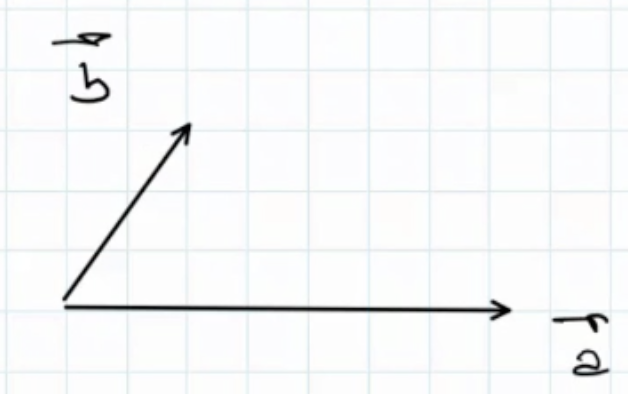
\includegraphics[width = 0.5 \textwidth]{lezione1/images/somma1.png}
\caption{passo 1, rappresento i due vettori come segmenti di retta}
\label{fig:somma1}
\end{center}
\end{figure}

Il vettore somma viene definito attraverso la \textbf{regola del parallelogramma}. Prendiamo il segmento $b$ e portiamo la coda di questo segmento, in prossimità della punta del segmento $a$

\begin{figure}[h]
\begin{center}
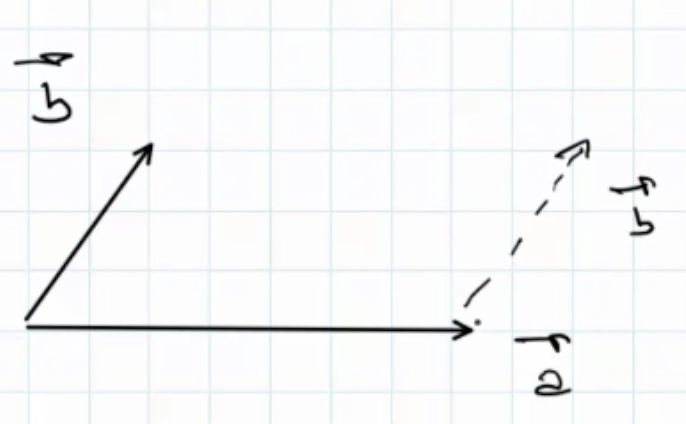
\includegraphics[width = 0.5 \textwidth]{lezione1/images/somma2}
\caption{passo 2, porto la coda di b sulla punta di a}
\label{fig:somma2}
\end{center}
\end{figure}

A questo punto, non ci resta che congiungere la coda di $a$ con la punta di $b$ e otterremo così il vettore somma $\overrightarrow{c}$

\begin{figure}[h]
\begin{center}
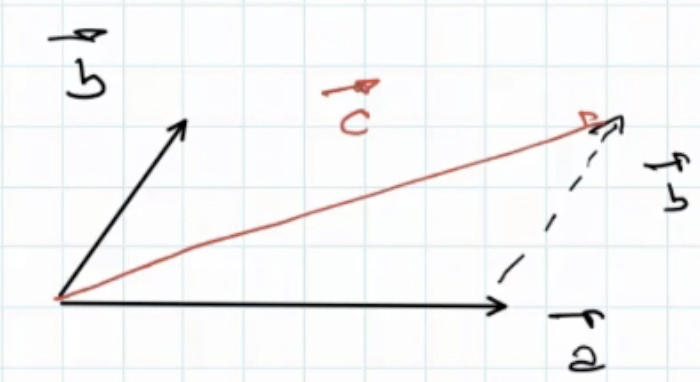
\includegraphics[width = 0.5 \textwidth]{lezione1/images/somma3}
\caption{passo 3, congiungo la coda di a con la punta di b}
\label{fig:somma3}
\end{center}
\end{figure}

\subsection{Differenza tra due vettori}
Siamo sotto le stesse ipotesi della somma; abbiamo quindi due vettori 
$\overrightarrow{a} $ e $\overrightarrow{b} $ che andiamo nuovamente a rappresentare come due segmenti orientati di retta. Com'è fatto il vettore 
$ \overrightarrow{d} = \overrightarrow{a} - \overrightarrow{b} $ ? 

\begin{figure}[h]
\begin{center}
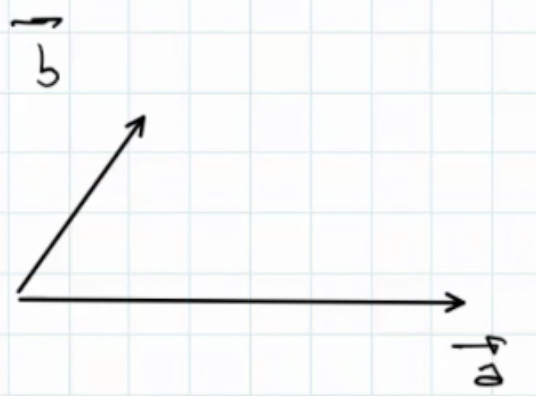
\includegraphics[width = 0.5 \textwidth]{lezione1/images/differenza1}
\caption{passo 1, rappresento i due vettori come segmenti di retta}
\label{fig:differenza1}
\end{center}
\end{figure}

La differenza tra due vettori $\overrightarrow{a} - \overrightarrow{b} $ può essere riscritta come la somma tra $\overrightarrow{a}$ e il vettore opposto a $\overrightarrow{b}$. Possiamo quindi scrivere che
$$\overrightarrow{d} = \overrightarrow{a} + (-\overrightarrow{b}) $$
Per fare la differenza, quindi, dobbiamo trovare il vettore opposto a 
$\overrightarrow{b}$ e poi facciamo la somma con la regola del parallelogramma vista sopra.

Ricordiamo che il vettore opposto a $\overrightarrow{b}$ ha stessa lunghezza e stessa direzione di $\overrightarrow{b}$, ma ha verso opposto.

\begin{figure}[h]
\begin{center}
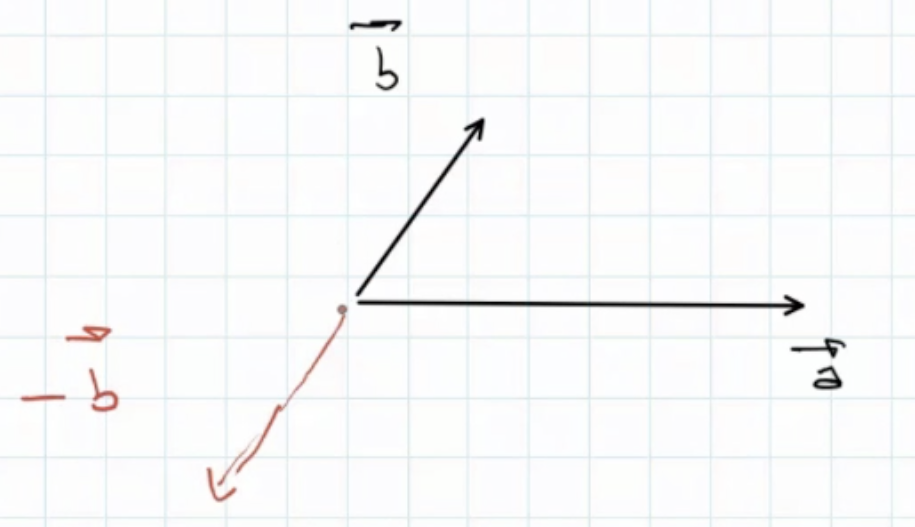
\includegraphics[width = 0.5 \textwidth]{lezione1/images/differenza2}
\caption{passo 2, trovo il vettore opposto a b}
\label{fig:differenza2}
\end{center}
\end{figure}
\newpage
Riutilizziamo adesso, la regola del parallelogramma vista sopra:

Quindi, mettiamo la coda del vettore opposto a $ \overrightarrow{b} $ sulla punta di
$\overrightarrow{a} $

\begin{figure}[h]
\begin{center}
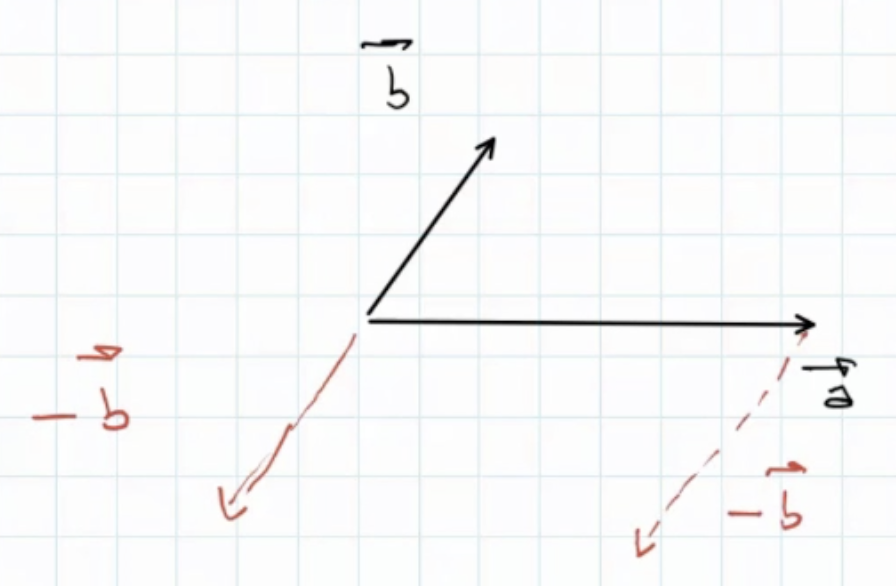
\includegraphics[width = 0.5 \textwidth]{lezione1/images/differenza3}
\caption{passo 3, porto la coda del vettore opposto a b sulla punta di a}
\label{fig:differenza3}
\end{center}
\end{figure}

Infine, congiungiamo la coda di $ \overrightarrow{a} $ con la punta di $- \overrightarrow{b}$ e otteniamo, così, il vettore differenza $\overrightarrow{d} $.

\begin{figure}[h]
\begin{center}
\includegraphics[width = 0.5 \textwidth]{lezione1/images/differenza4}
\caption{passo 4, congiungo la coda di a con la punta del vettore opposto a b}
\label{fig:differenza4}
\end{center}
\end{figure}

Volendo, si può fare la controprova, che ci fa capire se tutto è corretto:

Se prendiamo il vettore $ \overrightarrow{d} $ e il vettore $\overrightarrow{b}$, se li sommiamo con la regola del parallelogramma otteniamo
$$ \overrightarrow{d} + \overrightarrow{b} = \overrightarrow{a} $$

Fino ad adesso, abbiamo definito le operazioni tra i vettori con un metodo grafico; questo metodo, può andare bene se lavoriamo su un piano a due dimensioni. Man mano che aggiungiamo dimensioni, però, graficamente le cose si complicano.

\newpage

\subsection{La scomposizione di un vettore}
Supponiamo di lavorare sul piano a due dimensioni; sia $\overrightarrow{a} $ un vettore, e siano $\overrightarrow{u}_{r}$ ed $\overrightarrow{u}_{s}$ due vesori che mi definiscono due direzioni.

\begin{figure}[h]
\begin{center}
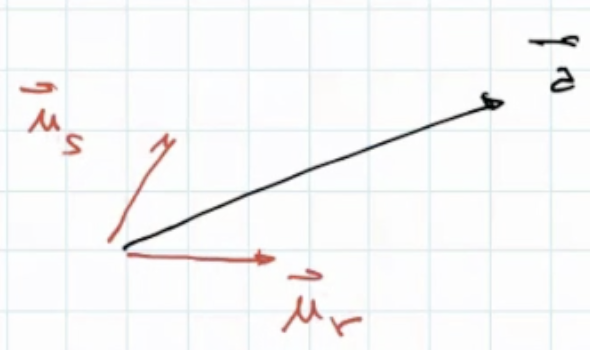
\includegraphics[width = 0.5 \textwidth]{lezione1/images/scomposizione1}
\label{fig:scomposizione1}
\end{center}
\end{figure}

Scomporre un vettore $\overrightarrow{a} $ significa scrivere tale vettore, come la somma di due vettori uno parallelo a $\overrightarrow{u}_{r}$ , l'altro parallelo a $\overrightarrow{u}_{s}$. Se indichiamo con $ \overrightarrow{a}_{r}$ e $ \overrightarrow{a}_{s}$ questi due vettori paralleli possiamo scrivere
$$ \overrightarrow{a} = \overrightarrow{a}_{r} + \overrightarrow{a}_{s} $$
In precedenza, abbiamo visto che un vettore può sempre essere scritto come il suo modulo, moltiplicato per il suo versore. Possiamo, quindi, riscrivere l'equazione sopra come
$$ \overrightarrow{a} = \overrightarrow{a}_{r} + \overrightarrow{a}_{s} = a_{r}\overrightarrow{u}_{r} + a_{s}\overrightarrow{u}_{s} $$ (dove $ \overrightarrow{u}_{r} $ e  $ \overrightarrow{u}_{s} $ sono i due versori che specificano direzioni e verso)
Fare la scomposizione di $\overrightarrow{a}$ vuol dire trovare $ \overrightarrow{a}_{r} $ e $ \overrightarrow{a}_{s} $

La cosa interessante è quando nel mio piano di riferimento, conosco una coppia di versori che sono perpendicolari tra di loro. La cosa si può estendere al piano con tre dimensioni: all'interno dello spazio tridimensionale, conosco una terna di versori perpendicolari tra loro. 
Questa terna di versori perpendicolari tra di loro, può essere indicata o con la notazione $$\lbrace\overrightarrow{u}_{x}, \overrightarrow{u}_{y},  \overrightarrow{u}_{z}\rbrace \quad oppure \quad \lbrace \overrightarrow{i}, \overrightarrow{j}, \overrightarrow{k}\rbrace $$
Le due notazioni sopra riportate sono equivalenti.
Questa terna, descrive tre versori perpendicolari uno con l'altro e prende anche il nome di \textbf{base ortonormale}.

Se abbiamo a disposizione una terna di questi versori, le componenti di un certo vettore $\overrightarrow{a}$ in queste tre direzioni, $\lbrace\overrightarrow{u}_{x}, \overrightarrow{u}_{y},  \overrightarrow{u}_{z}\rbrace \quad oppure \quad \lbrace \overrightarrow{i}, \overrightarrow{j}, \overrightarrow{k}\rbrace $, prendono anche il nome di \textbf{componenti cartesiane del vettore $\overrightarrow{a}$}

L'operazione do scomposizione di un vettore, quindi, mi fornisce le sue componenti cartesiane.

Possiamo fare anche la cosa inversa: se abbiamo a disposizione una terna di questi versori, anziché specificare un vettore disegnando un segmento orientato di retta, posso specificare questo vettore, fornendo quelle che sono le sue componenti cartesiane rispetto alla terna di versori.

Il vantaggio di specificare vettori dando le componenti cartesiane è: se conosciamo due vettori scritti in questo modo
\newpage
\begin{align*}
\overrightarrow{a} = a_{x} \overrightarrow{i} + a_{y} \overrightarrow{j} + a_{z} \overrightarrow{k} \\
 \overrightarrow{b} = b_{x} \overrightarrow{i} + b_{y} \overrightarrow{j} + b_{z} \overrightarrow{k}
\end{align*}
 
possiamo scrivere il vettore somma $\overrightarrow{c}$ di questi due vettori come somma fatta componente per componente delle sue componenti cartesiane:
$$ \overrightarrow{c} = (a_{x} + b_{x}) \overrightarrow{i} + (a_{y} + b_{y}) \overrightarrow{j} + (a_{z} + b_{z}) \overrightarrow{k} $$
Arrivati a questo punto possiamo riscrivere ancora il vettore somma $\overrightarrow{c}$ come
$$ \overrightarrow{c} = c_{x} \overrightarrow{i} + c_{y} \overrightarrow{j} + c_{z} \overrightarrow{k} $$

Allo stesso modo,  se volessimo trovare il vettore differenza, dovremmo fare la differenza (componente per componente) delle sue componenti cartesiane.

\subsection{Prodotto scalare e vettoriale}
Ci sono due tipi di prodotti tra vettori. Il primo, chiamato \textbf{prodotto scalare}, definisce il prodotto, in modo tale che il risultato ottenuto sia \textbf{ancora uno scalare}.

Il secondo, chiamato \textbf{prodotto vettoriale}, definisce il prodotto in modo tale che il risultato ottenuto sia un \textbf{vettore}.

\subsubsection{Prodotto scalare}
Siano $ \overrightarrow{a} $ e $ \overrightarrow{b} $ due vettori; sia $ \Theta $ l'angolo compreso tra $ \overrightarrow{a} $ e $ \overrightarrow{b} $

\begin{figure}[h]
\begin{center}
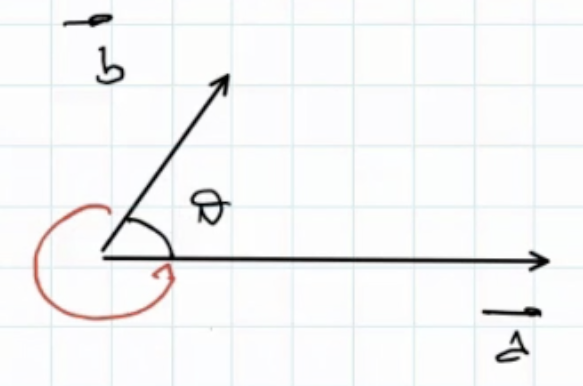
\includegraphics[width = 0.5 \textwidth]{lezione1/images/scalare1}
\label{fig:scalare1}
\end{center}
\end{figure}

Sia $ s $ il risultato del prodotto scalare; tale prodotto viene indicato come
$$ s = \overrightarrow{a} \prodscal \overrightarrow{b} $$
Notare che, visto che $s$ è uno scalare, non dobbiamo mettergli la freccia sopra.

Definiamo il prodotto scalare tra $ \overrightarrow{a} $ e $\overrightarrow{b} $ come il prodotto tra il modulo di $\overrightarrow{a} $ , il modulo di $ \overrightarrow{b} $ e il coseno dell'angolo compreso tra i due vettori.
$$ s = \overrightarrow{a} \prodscal \overrightarrow{b} = a \, b \, \cos \Theta $$
È importante ricordare che:
$$ \cos \Theta = 0 \quad  se \, \,  \Theta = (2 n + 1) \frac{\pi}{2} $$
cioè: $ \cos \Theta = 0 $ se $ \Theta $ è un multiplo dispari di $ \frac{\pi}{2} $, quindi $s$, (il prodotto scalare tra $\overrightarrow{a}$ e $\overrightarrow{b}$), è uguale a 0 se:
$$ a = 0 \quad o\,p\,p\,u\,r\,e \quad b = 0 \quad o\,p\,p\,u\,r\,e \quad \cos \Theta = 0 \, \, o\,v\,v\,e\,r\,o \,\,\Theta = (2n+1) \frac{\pi}{2} $$
Un'altra cosa importante da sapere che viene dalla trigonometria è:
$$ \cos(2 \pi - \Theta) = \cos \Theta $$
Fare il $ cos(2 \pi - \Theta) $ vuol dire fare il coseno dell'angolo disegnato in rosso nella figura di pagina precedente (cioè il coseno dell'angolo che va da $\overrightarrow{b} $ ad $\overrightarrow{a} $ .

Se devo fare, quindi, il prodotto scalare tra $ \overrightarrow{b} $ ed $ \overrightarrow{a} $ , questo sarà uguale a:
$$ s = \overrightarrow{b} \prodscal \overrightarrow{a} = b\, a \cos(\pi - \Theta) = b \, a \cos \Theta $$
Riassumendo,  il prodotto scalare $\overrightarrow{b} \prodscal \overrightarrow{a} $ è uguale al modulo di $\overrightarrow{b}$ per il modulo di $ \overrightarrow{a} $ per il coseno di $ \Theta $
Possiamo, quindi,  affermare che
$$ \overrightarrow{a} \prodscal \overrightarrow{b} = \overrightarrow{b} \prodscal \overrightarrow{a} $$ 
Ciò vuol dire \textbf{che per il prodotto scalare vale la proprietà commutativa}.  \\

Vediamo, adesso, come si fa a calcolare il prodotto scalare utilizzando le componenti cartesiane dei vettori.
Sia $\lbrace \overrightarrow{i},  \overrightarrow{j}, \overrightarrow{k} \rbrace $ una terna di versori, e siano $\overrightarrow{a}$ e $ \overrightarrow{b} $ due vettori così definiti:
\begin{align*}
 \overrightarrow{a} = a_{x} \overrightarrow{i} + a_{y} \overrightarrow{j} + a_{z} \overrightarrow{k} \\
 \overrightarrow{b} = b_{x} \overrightarrow{i} + b_{y} \overrightarrow{j} + b_{z} \overrightarrow{k}
 \end{align*} 
 
Per fare il prodotto scalare tra questi due vettori, ogni componente cartesiana del vettore $ \overrightarrow{a} $ va moltiplicata per tutte le componenti del vettore $\overrightarrow{b} $. In pratica dovremmo calcolare
$$ a_{x} \overrightarrow{i} b_{x}\overrightarrow{i} + a_{x} \overrightarrow{i} b_{y}\overrightarrow{j} + a_{x} \overrightarrow{i} b_{z}\overrightarrow{k} + a_{y} \overrightarrow{j} b_{x}\overrightarrow{i} + a_{y} \overrightarrow{j} b_{y}\overrightarrow{j} + a_{y} \overrightarrow{j} b_{z}\overrightarrow{k} + \cdots  $$
Si continua in questo modo e  arriva fino a
$$ + \,  \cdots \, + a_{z} \overrightarrow{k} b_{z} \overrightarrow{k} $$

Otteniamo così 9 termini. Se osserviamo quello che abbiamo fatto, però, ci accorgiamo che stiamo facendo il prodotto tra uno scalare (la componente) e un versore. La cosa importante da capire, quindi, è quanto fa il prodotto scalare di un versore per un altro versore. In pratica dobbiamo vedere come è fatto il prodotto scalare tra $\overrightarrow{i},  \overrightarrow{j}$ e $\overrightarrow{k}$ uno con gli altri.

\subsubsection{Prodotto scalare tra versori}
Vediamo quanto fa $\overrightarrow{i} \prodscal \overrightarrow{i} $
Questa quantità è uguale al modulo di $\overrightarrow{i}$ per il modulo di $\overrightarrow{i} $ per il coseno dell'angolo compreso tra $ \overrightarrow{i} $ e $\overrightarrow{i}$ .
Sappiamo che l'angolo compreso tra $ \overrightarrow{i} $ e se stesso vale 0. Possiamo scrivere quindi che:

\begin{align*}
\overrightarrow{i} \prodscal \overrightarrow{i} = 1 \cdot 1 \cdot \cos 0 = \\
= 1 \cdot 1 \cdot 1 = 1 
\end{align*}

quindi:
$$ \overrightarrow{i} \prodscal \overrightarrow{i} = 1$$
inoltre:
$$ \overrightarrow{i} \prodscal \overrightarrow{i} = \overrightarrow{j} \prodscal \overrightarrow{j} = \overrightarrow{k} \prodscal \overrightarrow{k} = 1 $$

Stesso ragionamento vale per tutti gli altri prodotti:

\begin{align*}
\overrightarrow{i} \prodscal \overrightarrow{j} = 1 	\cdot 1 \cdot \cos \frac{\pi}{2} = \\
 = 1 \cdot 1 \cdot 0 = 0
\end{align*}

quindi:
$$ \overrightarrow{i} \prodscal \overrightarrow{j} = 0 $$

inoltre:

\begin{align*}
\overrightarrow{i} \prodscal \overrightarrow{j} = \overrightarrow{i} \prodscal \overrightarrow{k} = \overrightarrow{j} \prodscal \overrightarrow{k} = 0 \\
\overrightarrow{j} \prodscal \overrightarrow{i} = \overrightarrow{k} \prodscal \overrightarrow{i} = \overrightarrow{k} \prodscal \overrightarrow{j} = 0
\end{align*}

Possiamo dire che la regola è: \textbf{quando facciamo il prodotto di un versore per se stesso otteniamo 1, quando facciamo il prodotto di un versore per un versore differente otteniamo 0} .

Questo vuol dire che, quando dobbiamo fare il prodotto scalare tra due vettori definiti con le componenti cartesiane,  di quei 9 termini visti prima, tutti quelli che coinvolgono prodotti tra versori differenti, si annullano. Gli unici termini che "sopravvivono", sono quelli ottenuti da prodotti tra versori differenti. Il prodotto scalare, quindi è uguale a:

$$ s =\overrightarrow{a} \prodscal \overrightarrow{b} = a_{x} b_{x} + a_{y} b_{y} + a_{z} b_{z} $$

Possiamo dire, anche, che il prodotto scalare tra due vettori espressi tramite le loro componenti cartesiane, è dato dalla \textbf{somma dei prodotti che hanno lo stesso indice}.

Notare che se facciamo il prodotto scalare di un vettore per se stesso otteniamo:
$$ \overrightarrow{a} \prodscal \overrightarrow{a} = {a^{2}}_{x} + {a^{2}}_{y} + {a^{2}}_{z} $$
Questa quantità rappresenta il quadrato della lunghezza del vettore. Quindi, il prodotto scalare di un vettore per se stesso, non ci fornisce nient'altro che la somma dei quadrati delle componenti cartesiane (è anche chiamato modulo quadro di $\overrightarrow{a} $). Infatti, possiamo riscrivere questa quantità come:
$$ \overrightarrow{a} \prodscal \overrightarrow{a} = {a^{2}}_{x} + {a^{2}}_{y} + {a^{2}}_{z} = a^{2} $$

Tornando a quello che abbiamo visto in precedenza sui versori, se dato un vettore $\overrightarrow{a} $, se abbiamo bisogno di trovare il suo versore $ \overrightarrow{u} $ , dobbiamo calcolare il modulo del vettore, prendere l'inverso e moltiplicare questo scalare per il vettore stesso. 
$$ \overrightarrow{u} = \frac{1}{a} \overrightarrow{a} $$
Adesso sappiamo che per trovare il versore di $\overrightarrow{a}$ possiamo calcolare il modulo quadro di $ \overrightarrow{a }$, farne la radice quadrata e infine fare l'inverso e moltiplicarlo per $\overrightarrow{a}$

\begin{align*}
\overrightarrow{u} = \frac{1}{\sqrt{ \overrightarrow{a} \prodscal \overrightarrow{a}}} \overrightarrow{a} = \\
 \frac{1}{\sqrt{a^{2}}} \overrightarrow{a} \quad \overrightarrow{u} = \frac{1}{a} \overrightarrow{a}  
\end{align*}

\subsubsection{Prodotto vettoriale}
Come detto prima, dati due vettori, il prodotto vettoriale tra i due restituisce ancora un vettore.

Siano $ \overrightarrow{a}$ e $\overrightarrow{b} $ due vettori, sia $ \Theta $ l'angolo compreso tra $ \overrightarrow{a} $ e $ \overrightarrow{b} $

\begin{figure}[h]
\begin{center}
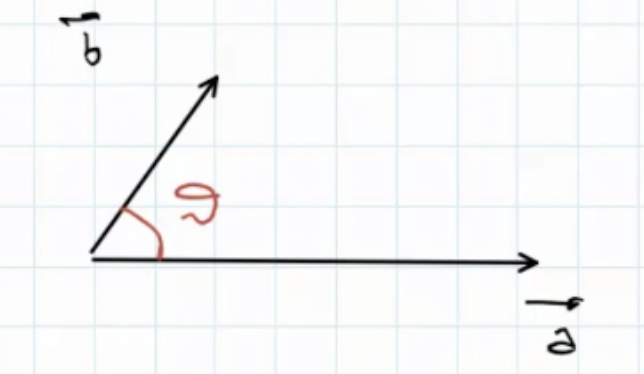
\includegraphics[width = 0.5 \textwidth]{lezione1/images/vettoriale1}
\label{fig:vettoriale1}
\end{center}
\end{figure}

Sia $ \overrightarrow{c} $ il vettore che otteniamo dal prodotto vettoriale tra $ \overrightarrow{a} $ e $ \overrightarrow{b} $ , indicheremo allora il prodotto vettoriale nel modo seguente:
$$ \overrightarrow{c} = \overrightarrow{a} \times \overrightarrow{b} $$

Visto che $ \overrightarrow{c} $ è un vettore, come ormai sappiamo, dobbiamo definirlo dando un modulo, una direzione e un verso.

il modulo di $ \overrightarrow{c} $ è uguale al modulo di $ \overrightarrow{a} $ per il modulo di $ \overrightarrow{b} $ per il seno dell'angolo compreso tra $\overrightarrow{a}$ e $ \overrightarrow{b} $ (che qui abbiamo chiamato $ \Theta $ )
$$ c = a \, b \,  \sin \Theta $$

\newpage
La rappresentazione geometrica del modulo di $ \overrightarrow{c} $ è significativa. $\overrightarrow{b} \sin \Theta $ è la quantità riportata nella figura qui sotto.

\begin{figure}[h]
\begin{center}
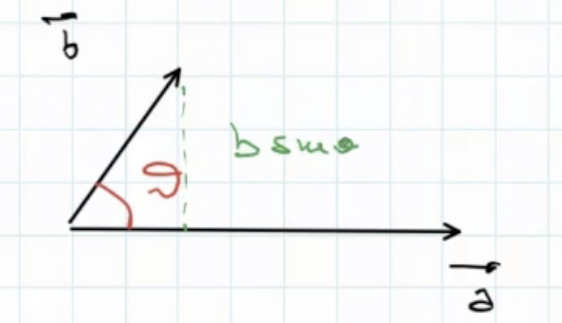
\includegraphics[width = 0.5 \textwidth]{lezione1/images/vettoriale2}
\label{fig:vettoriale2}
\end{center}
\end{figure}

La rappresentazione geometrica del modulo del prodotto vettoriale è l'area del parallelogramma che ha come lati $ \overrightarrow{a} $ e $  \overrightarrow{b} $

\begin{figure}[h]
\begin{center}
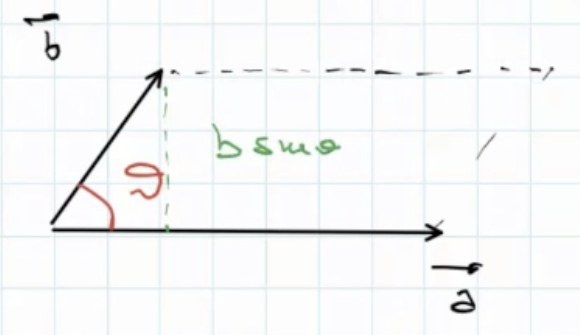
\includegraphics[width = 0.5 \textwidth]{lezione1/images/vettoriale3}
\caption{Interpretazione geometrica del modulo del prodotto vettoriale}
\label{fig:vettoriale3}
\end{center}
\end{figure}

Dobbiamo ancora specificare, però, direzione e verso del vettore $ \overrightarrow{c} = \overrightarrow{a} \times \overrightarrow{b} $.

La direzione è \textbf{perpendicolare al piano definito dai vettori $  \overrightarrow{a} $ e $ \overrightarrow{b} $} .

Per quanto riguarda il verso, è convezione assegnare il \textbf{verso} del vettore $ \overrightarrow{c} $ in base alla \textbf{regola della mano destra}.

Secondo questa regola,  mettiamo la nostra mano destra e la orientiamo in modo che:

\begin{itemize}
\item il pollice sia diretto lungo $ \overrightarrow{a} $
\item l'indice sia diretto lungo $ \overrightarrow{b} $
\item facendo i 2 passi precedenti, in automatico il medio sarà diretto lungo il verso di $ \overrightarrow{c} $
\end{itemize}

\newpage

\begin{figure}[h]
\begin{center}
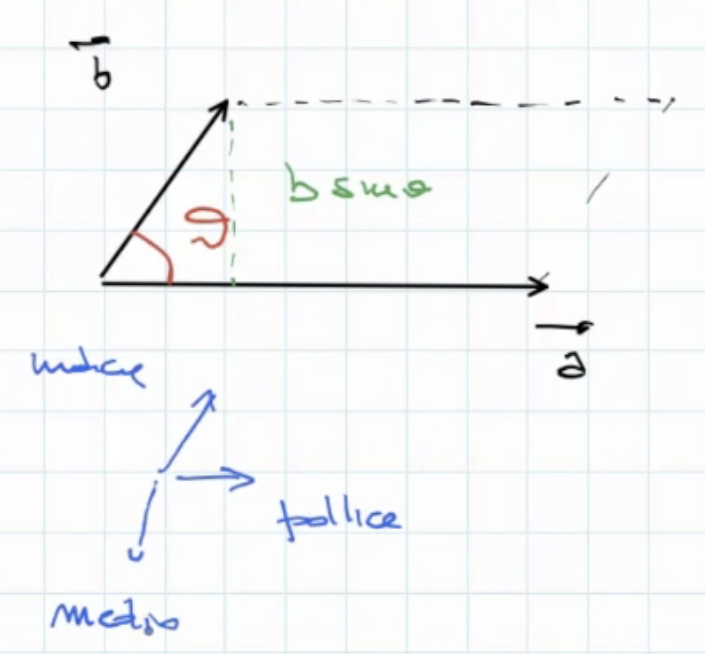
\includegraphics[width = 0.5 \textwidth]{lezione1/images/manodx}
\caption{Spiegazione regola della mano destra}
\label{fig:manodx}
\end{center}
\end{figure}

Notare che, nel caso rappresentato in figura, il dito medio "esce dal piano".

Ricapitolando, possiamo dire che: $\overrightarrow{c} = \overrightarrow{a} \times \overrightarrow{b} $ ha:

\begin{itemize}
\item modulo uguale a $ a \cdot b \sin $ angolo compreso tra $ \overrightarrow{a} $ e $ \overrightarrow{b} $
\item direzione perpendicolare al piano definito da $ \overrightarrow{a} $ e $ \overrightarrow{b} $
\item verso assegnato secondo la regola della mano destra
\end{itemize}

Vediamo, adesso, i casi in cui il prodotto vettoriale è nullo.
Il prodotto vettoriale è nullo se:

$ c = 0 $ sappiamo che $ c = 0 $ quando $ a = 0 $ oppure $ b = 0 $ oppure $ \sin \Theta = 0 $

Inoltre sappiamo che $ \sin \Theta = 0 $ quando: 
$$ \sin \Theta = 0 \quad s\,e \quad \Theta = 2n \cdot \frac{\pi}{2} = n\pi $$
Cioè il $ \sin \Theta = 0 $ quando $ \Theta $ è un multiplo pari di $ \frac{\pi}{2} $ oppure è un multiplo intero di $ \pi $ . Notare che l'angolo compreso tra $ \overrightarrow{a} $ e $ \overrightarrow{b} $ è un multiplo intero di $ \pi $ , quando $\overrightarrow{a} $ e $ \overrightarrow{b} $ giacciono sulla stessa retta; in particolare quando $ \overrightarrow{a} $ e $ \overrightarrow{b} $ hanno la stessa direzione e stesso verso, oppure hanno stessa direzione ma verso opposto. In questi casi, quindi, il prodotto vettoriale è 0. Se pensiamo all'interpretazione geometrica vista in precedenza, il prodotto vettoriale è nullo perché l'altezza del parallelogramma è 0.

Vediamo ancora una proprietà: sappiamo che il modulo di $ \overrightarrow{c} $ è uguale a:
$$ c = ab \sin \Theta  $$
dove, come detto prima, l'angolo $ \Theta $ è l'angolo che va dal vettore $ \overrightarrow{a} $ al vettore $ \overrightarrow{b} $ . Questo angolo è legato all'angolo che va dal vettore $ \overrightarrow{b} $ al vettore $ \overrightarrow{a} $ dalla seguente relazione:
\newpage

Se l'angolo che va da $ \overrightarrow{a} $ a $ \overrightarrow{b} $ vale $ \Theta $ , allora l'angolo  che va da $ \overrightarrow{b} $ ad $ \overrightarrow{a} $ è uguale a $ 2 \pi - \Theta $

\begin{figure}[h]
\begin{center}
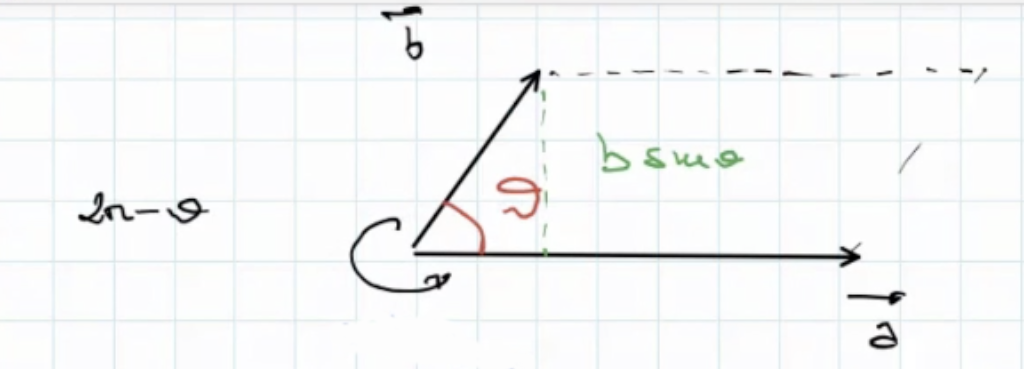
\includegraphics[width = 0.5 \textwidth]{lezione1/images/vettoriale4}
\label{fig:vettoriale4}
\end{center}
\end{figure}

Se facciamo quindi il prodotto vettoriale $ \overrightarrow{c}^{1} =  \overrightarrow{b} \times \overrightarrow{a} $ , il modulo di $\overrightarrow{c}^{1} $  è uguale a:

$$ c^{1} = b\, a \sin(2 \pi - \Theta) $$

Ma siccome il $ \sin(2 \pi - \Theta) $ è l'opposto del $ \sin \Theta $ , possiamo scrivere:
$$ c^{1} = b\, a \sin(2 \pi - \Theta) = -b \, a \sin \Theta $$

Per quanto riguarda la direzione di $ \overrightarrow{c}^{1} $ , anche lui è perpendicolare al piano definito da $ \overrightarrow{a} $ e $ \overrightarrow{b} $ .
In altre parole, il modulo e la direzione di $ \overrightarrow{c}^{1} $ sono uguali a quelli del vettore $ \overrightarrow{c} $. Per quanto riguarda il verso, invece, se applichiamo la regola della mano destra (pollice lungo $\overrightarrow{b} $ e indice lungo $ \overrightarrow{a} $ ), otteniamo che il verso di $\overrightarrow{c}^{1} $ l'opposto di quello di $\overrightarrow{c} $ . Possiamo, quindi, scrivere che
$$ \overrightarrow{b} \times \overrightarrow{a} = - \overrightarrow{a} \times \overrightarrow{b} $$

Vediamo, adesso, come si fa a calcolare il prodotto vettoriale tra $ \overrightarrow{a} $ e $ \overrightarrow{b} $ se abbiamo specificato questi due vettori con le loro componenti cartesiane.

Siano $ \overrightarrow{a} $ e $\overrightarrow{b} $ due vettori definiti come

\begin{align*}
\overrightarrow{a} = a_{x} \overrightarrow{i} + a_{y} \overrightarrow{j} + a_{z}\overrightarrow{k} \\
\overrightarrow{ b} = b_{x} \overrightarrow{i} + b_{y} \overrightarrow{j} + b_{z} \overrightarrow{k} 
\end{align*}

Anche in questo caso dobbiamo fare il prodotto vettoriale tra i termini di $\overrightarrow{a} $ e i termini di $ \overrightarrow{b} $ e dobbiamo ricordaci che "la parte che interviene" sul risultato del prodotto, sono i prodotti vettoriali tra i versori.

Dobbiamo capire, quindi, quanto valgono i prodotti vettoriali tra versori.

\subsubsection{Prodotto vettoriale tra versori}
Cominciamo calcolando quanto vale il prodotto vettoriale $ \overrightarrow{i} \times \overrightarrow{i} $: il risultato di questo prodotto è un vettore che ha:
modulo pari al modulo di $\overrightarrow{i} $ per il modulo di $ \overrightarrow{i} $ per il seno dell'angolo compreso tra $ \overrightarrow{i} $ e se stesso
$$ \overrightarrow{i} \times \overrightarrow{i} = 1 \cdot 1 \cdot \sin 0 $$
Sappiamo che $ \sin 0 = 0 $ quindi possiamo scrivere:
\begin{align*}
	\overrightarrow{i} \times \overrightarrow{i} = 1 \cdot 1 \cdot \sin 0 = 1 \cdot 1 \cdot 0 \\
	\overrightarrow{i} \times \overrightarrow{i} = 0
\end{align*}

Inoltre
$$ \overrightarrow{1} \times \overrightarrow{i} = \overrightarrow{j} \times \overrightarrow{j} = \overrightarrow{k} \times \overrightarrow{k} = 0 $$

Utilizzando lo stesso ragionamento, vediamo quanto valgono gli altri prodotti.
$$ \overrightarrow{i} \times \overrightarrow{j} = 1 \cdot 1 \cdot \sin \frac{\pi}{2} $$
Essendo due versori, $ \overrightarrow{i} $ e $ \overrightarrow{j} $ hanno modulo pari a 1. Siccome questi due versori sono perpendicolari tra loro, l'angolo che va da $\overrightarrow{i} $ a $\overrightarrow{j} $ vale $ \frac{\pi}{2} $ .  Sappiamo che il $ \sin \frac{\pi}{2} = 1 $ , quindi possiamo scrivere:
\begin{align*}
\overrightarrow{i} \times \overrightarrow{j} = 1 \cdot 1 \cdot \sin \frac{\pi}{2} = 1 \cdot 1 \cdot 1 \\
\overrightarrow{i} \times \overrightarrow{j} = 1
\end{align*}

Abbiamo capito, quindi, che $ \overrightarrow{i} \times \overrightarrow{j} $ è un vettore che ha modulo uguale a 1. Per quanto riguarda il verso, dobbiamo applicare la regola della mano destra.

Per applicare la regola della mano destra, dobbiamo decidere in che modo sono orientati i versori $ \overrightarrow{i} , \overrightarrow{j} $ e $ \overrightarrow{k} $ . Solitamente, la convenzione che si usa è la seguente:

\begin{figure}[h]
\begin{center}
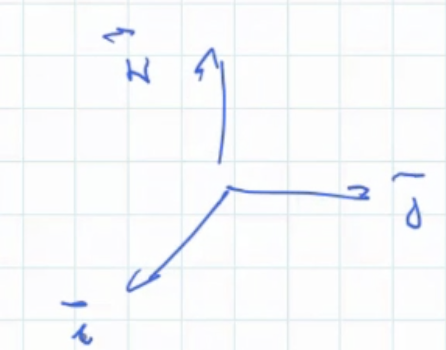
\includegraphics[width = 0.5 \textwidth]{lezione1/images/convenzione versori}
\label{fig:convenzione}
\caption{Convenzione orientamento versori}
\end{center}
\end{figure}

Utilizzando la regola della mano destra, mettiamo il pollice lungo $ \overrightarrow{i} $ e l'indice lungo $ \overrightarrow{j} $ ; così facendo, il verso (che è sempre indicato dal medio), sarà lungo $ \overrightarrow{k} $ .

Possiamo scrivere, quindi, che il verso del prodotto vettoriale
$$ \overrightarrow{i} \times \overrightarrow{j} = \overrightarrow{k} $$

Analogamente possiamo determinare i versi di tutti gli altri prodotti
\begin{align*}
\overrightarrow{i} \times \overrightarrow{j} = \overrightarrow{k} \\
\overrightarrow{j} \times \overrightarrow{k} = \overrightarrow{i} \\
\overrightarrow{k} \times \overrightarrow{i} = \overrightarrow{j}
\end{align*}
\newpage
Per ricordarci in maniera semplice questi prodotti, possiamo utilizzare questa figura

\begin{figure}[h]
\begin{center}
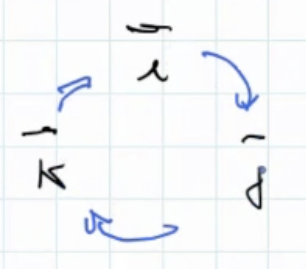
\includegraphics[width = 0.5 \textwidth]{lezione1/images/vettoriale5}
\label{fig:vettoriale5}
\end{center}
\end{figure}

Se percorriamo questa figura al contrario rispetto alle frecce otteniamo anche le altre combinazioni che hanno, però, \textbf{un segno meno davanti}
\begin{align*}
\overrightarrow{j} \times \overrightarrow{i} = - \overrightarrow{k} \\
\overrightarrow{k} \times \overrightarrow{j} = - \overrightarrow{i} \\
\overrightarrow{i} \times \overrightarrow{k} = - \overrightarrow{j}
\end{align*}

Ricapitolando, se la nostra base ortonormale è composta da $ {\overrightarrow{i}, \overrightarrow{j}, \overrightarrow{k}} $ se facciamo il prodotto vettoriale di un versore con se stesso otteniamo 0 , se invece facciamo il prodotto vettoriale tra versori differenti abbiamo che:
\begin{itemize}
\item se percorriamo la figura in senso orario, otteniamo prodotti con un segno $ + $
\item se percorriamo la figura in senso antiorario, otteniamo prodotti con un segno $ - $
\end{itemize}

Infine, siccome i prodotti vettoriali di versori con se stessi fanno 0, dei 9 termini totali ne rimangono 6 e raccogliendoli rispetto ai versori otteniamo;
\begin{align*}
\overrightarrow{a} \times \overrightarrow{b} = ( a_{x} \overrightarrow{i} + a_{y}\overrightarrow{j} + a_{z} \overrightarrow{k}  ) \times ( b_{x} \overrightarrow{i} + b_{y} \overrightarrow{j} + b_{z} \overrightarrow{k} = \\
( a_{x} b_{y} - a_{y} b_{x} ) \overrightarrow{k} - ( a_{x} b_{z} - a_{z} b_{x} ) \overrightarrow{j} + ( a_{y} b_{z} - a_{z} b_{y} ) \overrightarrow{i}
\end{align*}
Un modo per memorizzare questa espressione è
$$ \overrightarrow{a} \times \overrightarrow{b} = \begin{bmatrix}
\overrightarrow{i} & \overrightarrow{j} & \overrightarrow{k} \\
a_{x} & a_{y} & a_{z} \\
b_{x} & b_{y} & b_{z}
\end{bmatrix}  $$
Il valore del prodotto vettoriale è rappresentato dal \textbf{determinante di questa matrice}.

$$ \overrightarrow{a} \times \overrightarrow{b} = \begin{bmatrix}
\overrightarrow{i} & \overrightarrow{j} & \overrightarrow{k} \\
a_{x} & a_{y} & a_{z} \\
b_{x} & b_{y} & b_{z}
\end{bmatrix}  
= ( a_{y} b_{z} - a_{z} b_{y} ) \overrightarrow{i} + ( a_{x} b_{y} - a_{y} b_{x} ) \overrightarrow{k} - ( a_{x} b_{z} - a_{z} b_{x} ) \overrightarrow{j}  $$

\section{Esercizio}
Svolgiamo il seguente esercizio per applicare quanto visto fino adesso.

Siano dati i vettori
\begin{align*}
\overrightarrow{a} = 4 \overrightarrow{i} + 3 \overrightarrow{j} \\
\overrightarrow{b} = \overrightarrow{i} + 2 \overrightarrow{j}
\end{align*}
Calcolare:
\begin{itemize}
\item il modulo di $ \overrightarrow{a} $ e di $ \overrightarrow{b} $
\item i versori corrispondenti alla direzione di $ \overrightarrow{a} $ e di $\overrightarrow{b} $
\item i vettori somma $ \overrightarrow{s} = \overrightarrow{a} + \overrightarrow{b} $ e differenza $ \overrightarrow{d} = \overrightarrow{a} - \overrightarrow{b} $
\item il prodotto scalare $ \overrightarrow{a} \prodscal \overrightarrow{b} $ e il prodotto vettoriale $ \overrightarrow{a} \times \overrightarrow{b} $
\end{itemize}

\subsubsection{Svolgimento}
Cominciamo a calcolare il modulo di $\overrightarrow{a}$

per calcolarlo, dalla teoria sappiamo che il modulo quadro di $ \overrightarrow{a} $ è la somma del quadrato delle componenti cartesiane
\begin{align*}
 a^{2} = {a^{2}}_{x} + {a^{2}}_{y} = \\
  4^{2} + 3^{2} = 25 \rightarrow a = \sqrt{a^{2}} \\
  a = \sqrt{25}\\
  a = 5
\end{align*}

Stesso ragionamento per il modulo di $ \overrightarrow{b} $
\begin{align*}
b^{2} = {b^{2}}^{x} + {b^{2}}_{y} = \\
1^{2} + 2^{2} = 5 \rightarrow b = \sqrt{b^{2}} \\
b = \sqrt{5}
\end{align*}

Avendo calcolato i moduli, adesso possiamo calcolare i versori corrispondenti alle direzioni. Chiamiamo $ \overrightarrow{u}_{a} $ il versore lungo la direzione di $ \overrightarrow{a} $ e $ \overrightarrow{u}_{b} $ quello lungo $ \overrightarrow{b} $ .
Per calcolare i versori, come abbiamo visto, calcoliamo i moduli (che già abbiamo), ne facciamo l'inverso e infine facciamo il prodotto scalare dell'inverso del modulo per il vettore di partenza:
\begin{align*}
\overrightarrow{u}_{a} = \frac{1}{a} \prodscal \overrightarrow{a} = \frac{1}{5} \prodscal (4\overrightarrow{i} + 3\overrightarrow{j}) 
\end{align*}

Volendo, possiamo finire qui, oppure se vogliamo fare le cose per bene scriviamo:
\begin{align*}
\overrightarrow{u}_{a} = \frac{1}{a} \prodscal \overrightarrow{a} = \frac{1}{5} \prodscal (4\overrightarrow{i} + 3\overrightarrow{j}) \\
\overrightarrow{u}_{a} = \frac{4}{5} \overrightarrow{i} + \frac{3}{5} \overrightarrow{j}
\end{align*}

Facciamo la stessa cosa per $ \overrightarrow{b} $
\begin{align*}
\overrightarrow{u}_{b} = \frac{1}{b} \prodscal \overrightarrow{b} = \frac{1}{\sqrt{5}} \prodscal (\overrightarrow{i} + 2\overrightarrow{j}) \\
\overrightarrow{u}_{a} = \frac{1}{\sqrt{5}} \overrightarrow{i} + \frac{2}{\sqrt{5}} \overrightarrow{j}
\end{align*}
Abbiamo, così, calcolato i versori.

Riscriviamo i due vettori per comodità
\begin{align*}
\overrightarrow{a} = 4 \overrightarrow{i} + 3 \overrightarrow{j} \\
\overrightarrow{b} = \overrightarrow{i} + 2 \overrightarrow{j}
\end{align*}

Calcoliamo vettore somma e vettore differenza:

Siccome abbiamo le componenti cartesiane dei due vettori, il vettore somma sarà dato dalla somma delle due componenti $ x $ e la somma delle due componenti $ y $
\begin{align*}
\overrightarrow{s} = \overrightarrow{a} + \overrightarrow{b} = ( 4 + 1 )\overrightarrow{i} + ( 3 + 2 ) \overrightarrow{j} \\
\overrightarrow{s} = 5 \overrightarrow{i} + 5 \overrightarrow{j}
\end{align*}

il vettore differenza sarà dato dalla differenza delle due componenti $ x $ e la differenza delle due componenti $ y $
\begin{align*}
\overrightarrow{d} = \overrightarrow{a} - \overrightarrow{b} = ( 4 - 1 )\overrightarrow{i} + ( 3 - 2 ) \overrightarrow{j} \\
\overrightarrow{d} = 3 \overrightarrow{i} + \overrightarrow{j}
\end{align*}

Calcoliamo, ora il prodotto scalare tra $ \overrightarrow{a} $ e $ \overrightarrow{b} $ :

Per calcolare questo prodotto, come abbiamo visto dalla teoria, basta fare la somma dei prodotti delle componenti con lo stesso indice.
\begin{align*}
\overrightarrow{a} \prodscal \overrightarrow{b} = a_{x} b_{x} + a_{y} b_{y} = 4 \cdot 1 + 3 \cdot 2 \\
\overrightarrow{a} \prodscal \overrightarrow{b} = 4 + 6 \\
\overrightarrow{a} \prodscal \overrightarrow{b} = 10
\end{align*}

Infine, calcoliamo il prodotto vettoriale tra $ \overrightarrow{a} $ e $ \overrightarrow{b} $ :
Per calcolarlo o usiamo l'espressione ricavabile dal determinate della matrice:
$$ \overrightarrow{a} \times \overrightarrow{b} = \begin{bmatrix}
\overrightarrow{i} & \overrightarrow{j} & \overrightarrow{k} \\
a_{x} & a_{y} & a_{z} \\
b_{x} & b_{y} & b_{z}
\end{bmatrix} $$
oppure, possiamo semplicemente fare il prodotto vettoriale tra le componenti, facendo attenzione ai prodotti tra versori (noi utilizziamo questo modo):
\begin{align*}
\overrightarrow{a} \times \overrightarrow{b} = ( 4 \overrightarrow{i} + 3 \overrightarrow{j} ) \times ( \overrightarrow{i} + 2 \overrightarrow{j} ) \\
\overrightarrow{a} \times \overrightarrow{b} = 4 \overrightarrow{i} \times \overrightarrow{i} + 4\overrightarrow{i} \times 2 \overrightarrow{j} + 3 \overrightarrow{j} \times \overrightarrow{i} + 3 \overrightarrow{j} \times 2 \overrightarrow{j} \\
\overrightarrow{a} \times \overrightarrow{b} = 0 + 8 \overrightarrow{i} \times \overrightarrow{j} + 3 \overrightarrow{j} \times \overrightarrow{i} + 0 \\
\overrightarrow{a} \times \overrightarrow{b} = 0 + 8\overrightarrow{i} \times \overrightarrow{j} - 3 \overrightarrow{i} \times \overrightarrow{j} + 0 \\
\overrightarrow{a} \times \overrightarrow{b} = 5 \overrightarrow{i} \times \overrightarrow{j} \\
\overrightarrow{a} \times \overrightarrow{b} = 5 \overrightarrow{k}
\end{align*}